\documentclass[12pt, a4paper, oneside]{mwart} % Z automatu 10pt w przypisach
\usepackage[utf8]{inputenc} % Znaki diakrytyczne z klawiatury
\usepackage[OT4]{fontenc} % OT4 ponizej nie dzialalo
\usepackage[plmath,MeX]{polski} % Ponoc lepsza polonizacja LaTeXa
%\usepackage[dvips]{graphicx}
\usepackage[pdftex]{color,graphicx} % Grafika w PDFowej formie
%\usepackage{dcolumn} % Wyrownywanie przecinka w tabelach
%\newcolumntype{d}[1]{D{.}{,}{#1}} % Typ kolumny do wyrownywania
%\usepackage{threeparttable} % Coby ladnie podpisac tabelki
%\usepackage{rotating} % for sidewaystable
\usepackage{subcaption}
\captionsetup{compatibility=false}

\usepackage[pdftex]{hyperref} % Zarzadza hiperlaczami w dokumencie, ostatni w preambule, dvips/pdftex zaleznie od wyjscia

\begin{document}
\title{
\includegraphics[width = 0.3 \textwidth]{wykresy/SGHlogotypCMYKpl.eps}\\
\bigskip
Zaawansowane Modelowanie Symulacyjne [234060-0723]\\ 
\bigskip
Saloon "Wild West"\\
Symulacja baru na Dzikim Zachodzie}
\author{Anna Chojnacka, 68729 \and
Michał Puchalski, 67827 \and
Paweł Sadłowski, 68404 }
\date{Warszawa, 4.06.2019}
\maketitle

\pagebreak

\section{Opis~organizacji}
Saloon „Wild West” to szczególny rodzaj baru proponujący należyty odpoczynek oraz rozrywkę strudzonym wędrowcom starego Zachodu. Bar nie ma sobie równych jeśli chodzi o najlepszą obsługę klientów. Jego barmani oraz barmanki mogą poszczycić się najlepszymi~w Kansas umiejętnościami nalewania trunków, a~przy~stołach pokerowych niejeden znużony robotnik czy rewolwerowiec stawia na~szali dorobek życia w~nadziei na~szybką fortunę. Aktualnie, w~związku z~otwarciem nowych salonów na drodze prowadzącej do Leavenworth, właściciel baru stoi przed ważnymi decyzjami, które zadecydują o~przyszłości saloonu.

\section{Opis problemu}
W związku z rosnącą konkurencją oraz spadkiem wizerunku baru, właściciel saloonu poszukuje odpowiedniej strategii, która pozwoli mu zachować opinię najlepszego baru na Dzikim Zachodzie, a~tym samym utrzymać klientelę, jak i~zwiększyć zysk z~interesu. Zakres analizy obejmuje ocenę wrażliwości wysokości ceny drinków w barze, jak i~polepszenia wystroju baru. Została również przeprowadzona analiza dotycząca wpływu liczby danej płci barmanów oraz ich wyglądu na końcowy zysk salonu.

\subsection{Szczegółowy scenariusz symulacji}
Salon jest otwarty przez pewną liczbę godzin na dobę. Właściciel baru rekomenduje przybliżanie odwiedzin kolejnych klientów poprzez proces Poissona. Każdy klient wybiera jedną z~dwóch opcji: bycie obsługiwanym za barem lub dołączenie do partyjki pokera. Na czas spędzony przy barze składa się długość trwania serwisu oraz --- o~ile klient jest obsługiwany przez kobietę --- długość flirtu z~personelem losowana z rozkładu jednostajnego. Dłuższy czas obsługi przez barmanki rekompensowany jest losowanym z~rozkładu Gamma napiwkiem, który powiększa zysk saloonu ponad standardową cenę napoju. Długość picia drinka opisuje rozkład wykładniczy. Jeżeli wszyscy barmani są zajęci, klient musi czekać w kolejce by zostać obsłużonym. Jeżeli czas oczekiwania na obsługę przy barze przekroczy próg cierpliwości klienta, z~pewnym prawdopodobieństwem klient rozpęta awanturę i~zacznie się strzelanina, w~przeciwnym razie będzie cierpliwie czekał dalej. Po wypiciu drinka klient może podjąć trzy decyzje: opuszczenie lokalu, wypicie następnej kolejki lub dołączenie się do partyjki pokera. Rozpoczęcie rozgrywki pokera jest możliwe, gdy przy stole zbierze się 5 graczy, a długość jednej partii wynosi 10 minut. Partia z~niewielkim prawdopodobieństwem może zakończyć~się jednym ze~skrajnych wyników --- szczęściarz, który właśnie niebotycznie się wzbogacił funduje wszystkim obecnym kolejkę bądź też przegrany, po stracie ostatnich wysupłanych z~kieszeni oszczędności, rozpoczyna strzelaninę. O~ile tylko nie nastąpi drugie z~wymienionych zdarzeń, wszyscy gracze podejmują następnie zwykłe decyzje o~ponownej grze, wypiciu drinka lub opuszczeniu salonu. Każda strzelanina przynosi spore straty salonowi w~wysokości minimum 50~dolarów, a~dodatkowo w~jej wyniku z~pewnym prawdopodobieństwem może zginąć uwielbiany przez gości pianista --- w~tej sytuacji dodatkowe straty wynoszą 450~dolarów. Jednakże rozpętaniu strzelaniny z~łatwością może zaprzestać szeryf. Odwiedza on~codziennie lokal o~losowej porze (rozkład jednostajny) i~przesiaduje wewnątrz przez godzinę, spokojnie ćmiąc fajkę. Pod jego obecność nigdy nie~dochodzi do strzelaniny. Z~uwagi na~konieczność udzielenia pomocy rannym i~uprzątnięcia lokalu, saloon musi zostać zamknięty --- strzelanina kończy symulację. We wszystkich analizach zostały przyjęty jednodniowy horyzont czasowy. Dla zapewnienia stabilności wyników wygenerowano 1000 symulacji dla każdego scenariusza.

\subsection{Struktura modelu}
Przybycie kolejnych klientów opisywane jest procesem Poissona, zatem czas pomiędzy odwiedzinami kolejnych gości losowany jest z~rozkładu wykładniczego o~średniej równej 25~minut. Wieczorową porą chętnych na~odpoczynek i~pogawędkę jest więcej --- od~godziny 20:00 kolejni klienci pojawiają się przeciętnie co~20~minut. Z~prawdopodobieństwem 90\% klient udaje się do~baru, w~pozostałych przypadkach siada przy~stole pokerowym, o~ile są~jeszcze wolne miejsca. Standardowy czas obsługi klienta wynosi 5~minut, przedłuży się on~jednak o~wartość z~rozkładu jednostajnego na~przedziale 0-15~minut, gdy rewolwerowiec ma~do czynienia z~barmanką, której spróbuje się przypodobać. Zysk na~sprzedaży jednego drinka wynosi 2~dolary, napiwki są~losowane z~rozkładu Gamma z~parametrami $k = 5, \theta = 1$, co~daje przeciętną wysokość napiwku równą 5~dolarów. Średni czas picia drinka wynosi 35~minut, zaś próg cierpliwości klientów został wyjściowo ustalony na~poziomie 15~minut. Prawdopodobieństwo awantury w~kolejce wynosi co~najmniej 3\% i~od~godziny~21:00 rośnie liniowo z~upływem czasu. Każdy ze~skrajnych wyników partii pokera występuje z~prawdopodobieństwem równym 2\%. Liczba graczy gotowych do~rozpoczęcia kolejnej partii jest losowana z~rozkładu jednostajnego, zawsze jednak przynajmniej jeden z~graczy rezygnuje z~dalszej gry. Po wypiciu drinka bądź zakończeniu rozgrywki w~pokera klient opuszcza saloon z~prawdopodobieństwem 10\%. Strzelanina jest tym groźniejsza, im więcej alkoholu zdążyli wypić obecni wewnątrz goście --- straty rosną logarytmicznie od~godziny 23:00. Końcowy wynik baru stanowi suma zysku ze sprzedanych drinków oraz napiwków pomniejszona o~ewentualne straty wynikłe w~razie strzelaniny.

\section{Wyniki analizy}
Wyniki przeprowadzonych symulacji, których podstawą było 1000 iteracji modelu, szacują średni przychód baru na poziomie 174.95 \$ na dzień, a odchylenie na poziomie 108.47 \$. Wykres \ref{wyk_przychod} ilustruje rozkład wysokości przychodu z jednodniowej działalności baru. Najwyższe odseteki zmiennej stanowią wartości z przybliżonego przedziału od 190 do 230\$.

\subsection{Liczba zatrudnionych barmanów}
Wyniki analizy jednoznacznie wskazują, że zatrudnianie kolejnych barmanek jest o wiele bardziej opłacalne niż zatrudnianie kolejnych barmanów. Posiadanie tylko męskiego personelu oznaczałoby dla baru przychód w wysokości od 95.85 do 182.05 \$, jednakże posiadanie tylko barmanek (w liczbie od 2 do 10) przyniosłoby dzienne przychody w wysokości od 117.17 \$ do aż 271.75 \$ (posiadanie tylko jednego pracownika, którym byłaby kobieta wiąże się ze stratami w wysokości 5.87 \$). Wnioski te można odczytać z analizy mapy cieplnej (rysunek \ref{wyk_barmani}), na której zilustrowano wysokość przychodu w zależności od zróżnicowania płciowego personelu. Wyraźnie widać, że zysk z działalności salonu znacznie szybciej rośnie, gdy zostaje zatrudniona kolejna barmanka. Warto rozważyć optymalną różnorodność płciową personelu przy założeniu, że bar zatrudnia $n$ barmanów (przy założeniu równych płac). Dokładne wyniki analizy można zaobserwować na mapie cieplnej (rysunek \ref{wyk_barmani2}). Im intensywniejszy odcień niebieskiego (czerwonego), tym wyższy wzrost (spadek) średniego zysku względem $n-1$ liczby zatrudnionych barmanów. Kolor biały wyznacza kombinacje nieoptymalne. Najbardziej optymalną strategią dla baru będzie zatrudnienie najpierw mężczyzny, a następnie zatrudnienie dwóch barmanek. Od $n =4$ do $n=9$ opłaca się salonowi posiadać już tylko żeński personel. Jednakże, zatrudnianie kolejnych barmanów powyżej $n=5$ będzie przynosił niewielkie zyski lub straty z działalności baru. 

\begin{figure}
\centering
\caption{Rozkład wysokości przychodu z działalności salonu}
\label{wyk_przychod}
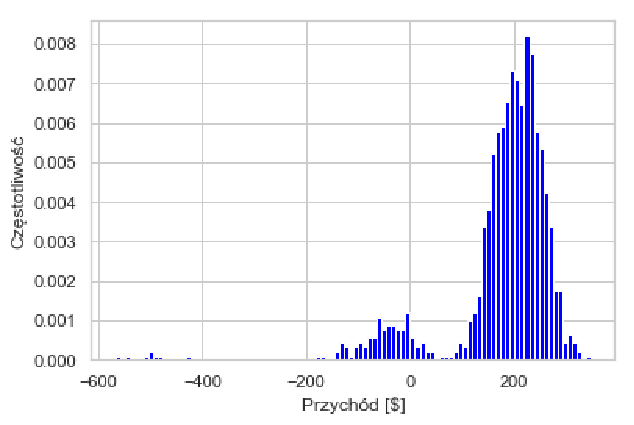
\includegraphics[width = 0.9\textwidth]{wykresy/histogram.pdf}
\end{figure}

\begin{figure}
\centering
\caption{Prognozowana wielkość przychodu w zależności od zróżnicowania płciowego personelu}
\label{wyk_barmani}
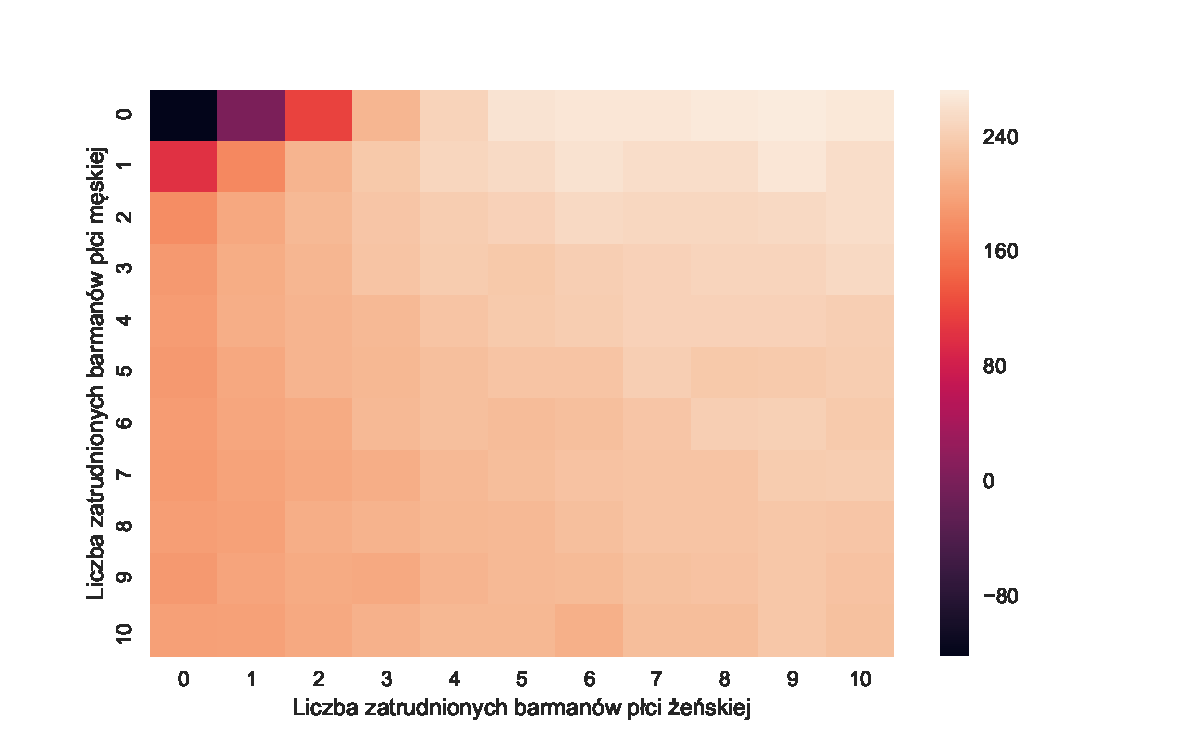
\includegraphics[width = 0.9\textwidth]{wykresy/barmani.pdf}
\end{figure}

\subsection{Wybór strategii cenowej}
Drugim parametrem, który ma znaczny wpływ na przychód salonu jest cena drinków na barze. Zostały wzięte pod uwagę trzy strategie cenowe: strategia umiarkowanych cen, gdzie koszt napoju wynosi 2 \$, strategia droższych drinków, gdzie koszt alkoholu wynosiłby 4 \$ oraz strategia tanich drinków, gdzie drink na barze kosztowałby tylko 1 \$. Wykres \ref{wyk_drinki} obrazuje prognozowany przeciętny przychód baru oraz jego odchylenie standardowe z zaproponowanych strategii. Prawie 1.87 razy wyższy przychód uzyskuje bar, jeśli obierze strategię droższych drinków zamiast strategii umiarkowanych cen, jednakże odchylenie standardowe dla korzystniejszej dochodowo strategii jest aż o 1.59 razy wyższe. Strategia tanich drinków jest nieopłacalna dla baru, gdyż przynosi straty, a jej odchylenie standardowe zmiennej jest największe.

\begin{figure}
\centering
\caption{Przecięta wielkość przychodu oraz jego odchylenie standardowe w zależności od przyjętej strategii cenowej}
\label{wyk_drinki}
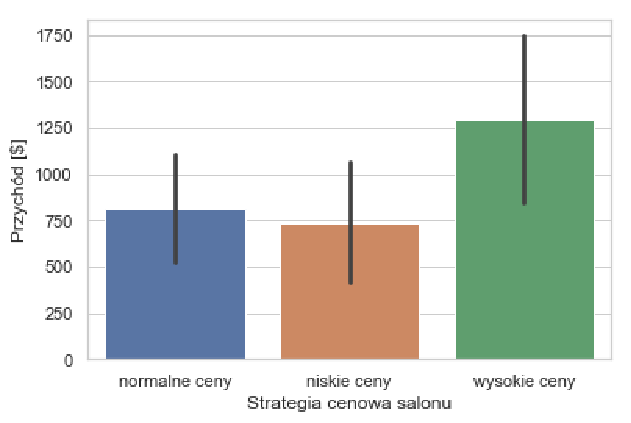
\includegraphics[width = 0.9\textwidth]{wykresy/drinki.pdf}
\end{figure}

\begin{figure}
\centering
\caption{Przecięta wielkość przychodu oraz jego odchylenie standardowe w zależności od wielkości stołu pokerowego}
\label{wyk_poker}
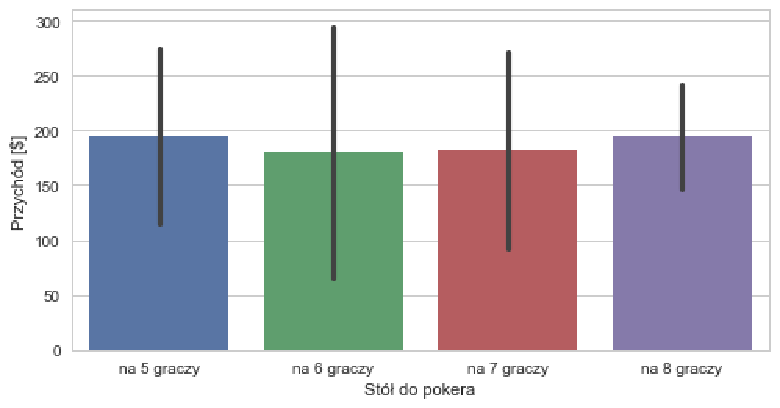
\includegraphics[width = 0.9\textwidth]{wykresy/poker.pdf}
\end{figure}

\subsection{Wybór optymalnej wielkości stołu do pokera}
Na przychód salonu znacznie również wpływa gra w pokera, a co za tym idzie wielkość stołu do gry oraz czas spędzony przez klientów na grze. Możliwy jest zakup czterech różnych rozmiarów stołu, przy którym kolejno pomieściłoby się od 5 do 8 graczy. Każdy dodatkowy gracz przy stole oznacza rozgrywkę trwającą 5 minut dłużej. Na wykresie \ref{wyk_poker} został zaprezentowany przeciętny przychód oraz odchylenie standardowe, dla każdej proponowanej wielkości stołu do pokera. Jak łatwo zauważyć, zwiększanie liczby dostępnych miejsc przy stole pokerowym nie prowadzi do znaczącego wzrostu przychodu (wzrost zysku z działalnosci pomiędzy najlepszą a najgorszą strategią wyniósł 9,7 \%). Dodatkowo należy pamiętać, że zakup większego stołu wiąże się prawdopodobnie z wyższymi kosztami mebla, co może być problematyczne dla właściciela baru, jeśli mebel uległby szybkiej eksploatacji czy zniszczeniu podczas strzelaniny.


\section{Analiza wrażliwości}
W ramach analizy wrażliwości rozważyliśmy dodatkowo trzy scenariusze: zatrudnianie przez bar ładniejszego personelu,

\subsection{Ładniejszy personel}
Rozważany przez nas scenariusz zakłada zatrudnianie przez właściciela baru tylko atrakcyjnego personelu. Zabieg ten przypuszczalnie zwiększył by czas flirtu klienta z barmanem z 15 do 25 minut, jednakże sam przeciętny napiwek również wzrósłby z 1 do 5 \$. Jak widać na wykresie \ref{wyk_personel}, średni przychód baru wzrasta aż o 42 \%, jeżeli właściciel salonu postanowi kierować się zaproponowaną strategią. Jednakże strategia ta będzie opłacalna w przypadku, jeśli zatrudnienie atrakcyjniejszego personelu nie będzie pociągało za sobą wyższych kosztów zatrudnienia, oraz tego, czy barmani będą szczerze rozliczać się z napiwków, a nie odkładać je do swoich kieszeni.

\begin{figure}
\centering
\caption{Przecięta wielkość przychodu oraz jego odchylenie standardowe w zależności od atrakcyjności personelu}
\label{wyk_personel}
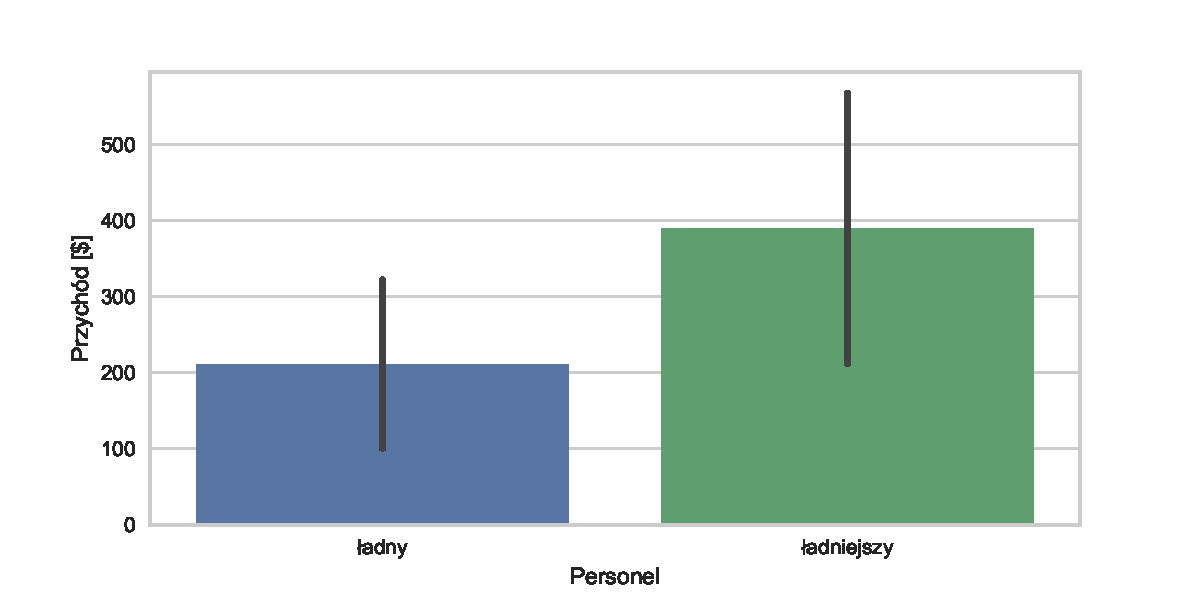
\includegraphics[width = 0.9\textwidth]{wykresy/personel.pdf}
\end{figure}

\subsection{Strzelaniny}

\subsection{Zajęcie w kolejce}


\section{Wnioski}

\begin{thebibliography}{9}
%\bibitem{slajdy}
%P.~Szufel, \emph{Zaawansowane Modelowanie Symulacyjne --- materiały do~wykładu}
\bibitem{law}
Averill~M.~Law, W.~David~Kelton,
\emph{Simulation Modeling \& Analysis},
McGraw-Hill, wyd.~piąte, 2015
\bibitem{sayama}
H.~Sayama, \emph{Introduction to the Modeling and Analysis of Complex Systems},
Open SUNY Textbooks, 2015
\bibitem{mielczarek}
Bożena~Mielczarek, \emph{Modelowanie symulacyjne w~zarządzaniu. Symulacja dyskretna},
Oficyna Wydawnicza Politechniki Wrocławskiej, Wrocław~2009
\end{thebibliography}

\end{document}